\ifx\wholebook\relax\else
\input{../Common.tex}
\input{../macroes.tex}
\begin{document}
\fi

\chapter{Loops and Variables}\label{ch:loopvar}

\begin{chapterfigure}
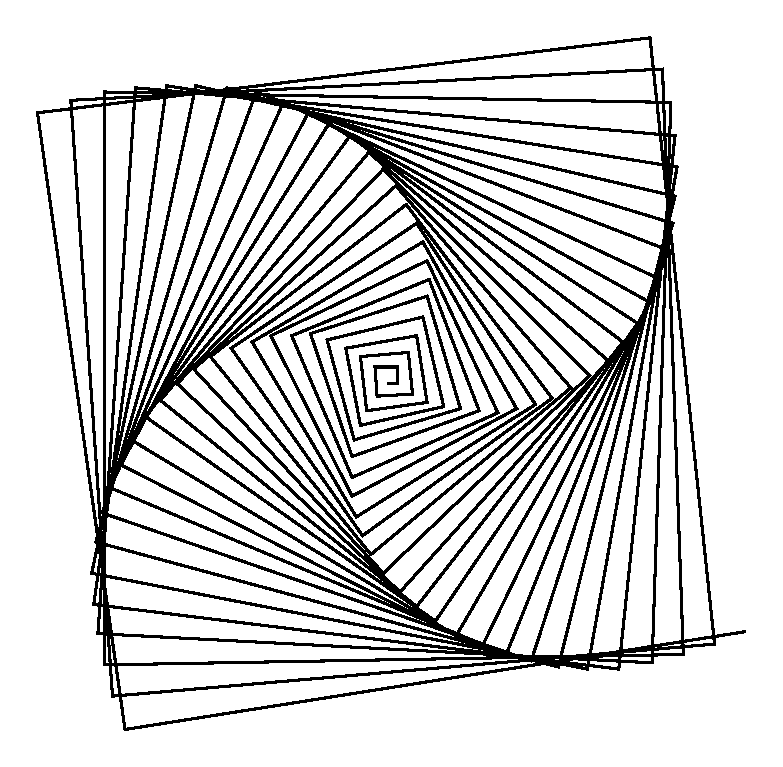
\includegraphics[width=0.9\linewidth]{varLoopsTitle}
\end{chapterfigure}


\hidden{
this is not the title
\begin{alltt}
| caro length angle |
caro := Turtle new.
length := 5.
angle := 179.
200 timesRepeat: [ caro go: length.
                 caro turnLeft: angle.
                 length := length + 5]

the one for the picture
| caro length angle |
caro := Turtle new.
length := 5.
angle := 178.
110 timesRepeat: [ caro go: length.
                 caro turnLeft: angle.
                 length := length + 3]
\end{alltt}}


In this chapter we present how variables and loops can be used
together. We start by analyzing a simple problem that
shows the need of using variables and loops together. We then
experiment with some other problems. 
%We introduce the new messages
%\ct{to:do:} and \ct{to:do:by:} that are more adapted to situations
%where sequences of numbers are needed.

\section{A Motivating Example}

Try to generate the strange stair shown in
Figure~\ref{fig:strangestair}. Start for example by generating a
normal stair and modify it. One of the problem that you should be
facing is that the length of each step is growing regularly.

\begin{figure}[!htbp]
\centerline{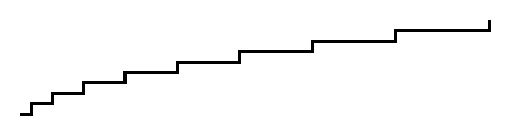
\includegraphics[width=12cm]{varLoopsFlatStair}}
\caption{A strange stair}
\label{fig:strangestair}
\end{figure}

One of the simplest solution is described by the
\scriptref{src:strange1} where the length of a step grows 10 by
10 pixels. However, such a solution is not satisfactory because we have to compute manually the length of the next step and that we have to
repeat stupidly the same sequence of messages.

\begin{scriptwithtitle}{Strange stair}\label{src:strange1}
| \caro |
\caro := \Turtle new.
\caro go: \bold{10}.
\caro turnLeft: 90.
\caro go: 5. 
\caro turnRight: 90.
\caro go: \bold{20}.
\caro turnLeft: 90.
\caro go: 5. 
\caro turnRight: 90.
\caro go: \bold{30}.
\caro turnLeft: 90.
\caro go: 5. 
\caro turnRight: 90.
\caro go: \bold{40}.
\caro turnLeft: 90.
\caro go: 5. 
\caro turnRight: 90.
...
\end{scriptwithtitle}

We would like to be able to use the power of variables and combined it with the one of loops. First avoiding to repeat the sequence of messages can be possible using the \timesRepeat method.  Second when we analyze the \scriptref{src:strange1} we see that the length of a step is the length of the preceding one plus 10. Here, 20 = 10 + 10, 30 = 20 + 10, 40 = 30 + 10,.... If we use the variable \ct{length} to represent the length of a step, we see that the length of the second step is the length of the first step plus 10, that the length of the third step is the length of the second step plus 10... We can express this by the
following expression \ct{length\ :=\ length\ + 10} which increases the value of the variable \ct{length} by 10.

Let's combine everything! Now if we take the script of a normal stair (\scriptref{src:normalstair}), introduce the variable \ct{length} we obtain a similar method and drawing
(\scriptref{src:normalstairlength}). Finally, if we change  \ct{length} value during each step of the loop, we obtain the stair we want (\scriptref{src:strangestair}).

\begin{scriptwithtitle}{A stair with normal steps}\label{src:normalstair}
| \caro |
\caro := \Turtle new.
10 timesRepeat: [\caro go: 10.
                \caro turnLeft: 90.
                \caro go: 5.
                \caro turnRight: 90]
\end{scriptwithtitle}

\begin{scriptwithtitle}{A stair with normal steps using \ct{length}}\label{src:normalstairlength}
| \caro \bold{length}|
\caro := \Turtle new.
\bold{length := 10.}
10 timesRepeat: [\caro go: \bold{length.}
                \caro turnLeft: 90.
                \caro go: 5.
                \caro turnRight: 90]
\end{scriptwithtitle}

\begin{scriptwithtitle}{The Solution}\label{src:strangestair}
| \caro \bold{length} |
\caro := Turtle new.
\bold{length := 10.}
10 timesRepeat: [\caro go: \bold{length}.
                \caro turnLeft: 90.
                \caro go: 5.
                \caro turnRight: 90.
                \bold{length := length + 10}]
\end{scriptwithtitle}


In the \scriptref{src:strangestair}, the sequence of messages in the loop, first make the robot go forward of a distance that is given by the value of the variable \ct{length}, the first time 10, then  the robot turns and draws the missing part of the stair, finally the value of the variable \ct{length} is increased by 10 and the loop restarts but with the variable \ct{length} having a value of 20. The same process is repeated 10 times.
Note that you should not forget the expression \ct{length\ :=\ length + 10} else the value of the variable would never change.

\begin{exonofig}
Change the last line of the loop for example put \ct{length\ :=\
length\ +\ 15}.  Change also the place where such a line occurs in the
loop. Can you explain what is happening when you move the last line of the
loop to the beginning of the loop?
\end{exonofig}

If you need more time to understand the solution proposed in the
\scriptref{src:strangestair}, we suggest you to look carefully at the value of the variable  variable \ct{length} in particular at the beginning and the end of the loop. You can also to simulate the messages sent. If necessary read again the Chapters~\ref{ch:variables}.



\section{Practicing: Mazes, Spirals and Other}
Now let us see how combining variables and loops helps us to solve
some other problems.
\begin{exofig}{varLoopsSquareStair}
Change the \scriptref{src:strangestair} to produce the picture shown on 
the right.
\end{exofig}


\begin{exofigwithsizeandtitle}[0.4]{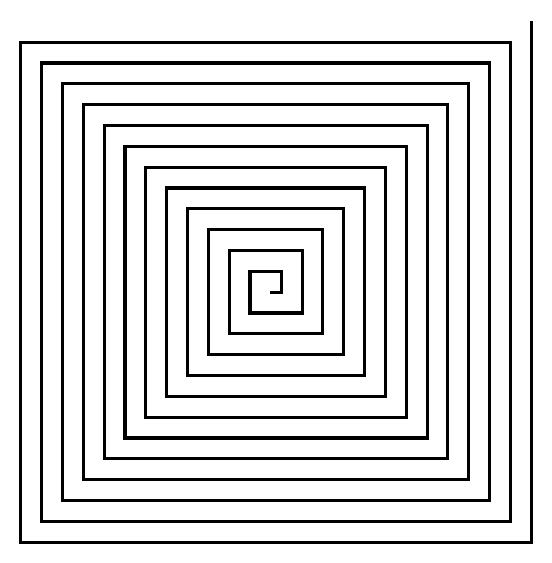
\includegraphics[width=6cm]{varLoopsMaze}}{Maze}\label{exo:maze}
Define a script that reproduces the drawing shown on the right. By turning from a different angle you should be able to recreate the first picture of the chapter as well as the  spiral shown in the Figure~\ref{fig:spiral}.
\end{exofigwithsizeandtitle}

\begin{figure}
\begin{center}
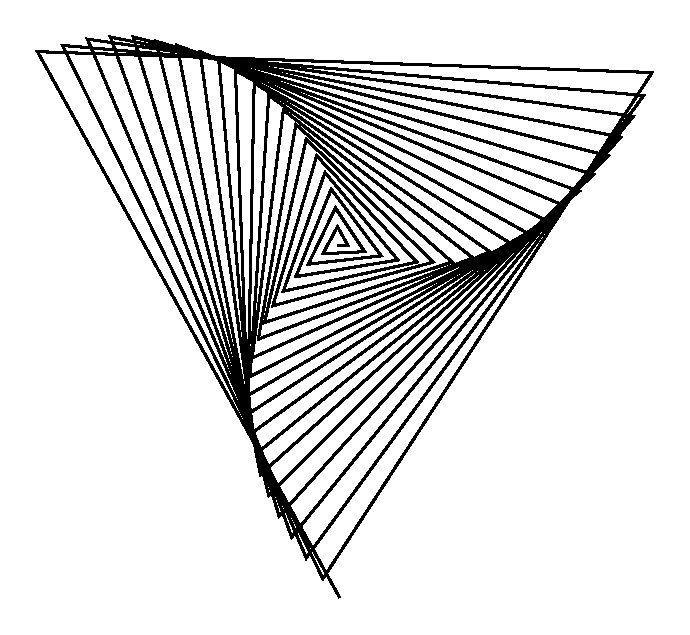
\includegraphics[width=8cm]{varLoopsSpiral121}
\caption{A nice spiral\label{fig:spiral}}
\end{center}
\end{figure}

\begin{exofigwithsizeandtitle}[0.5]{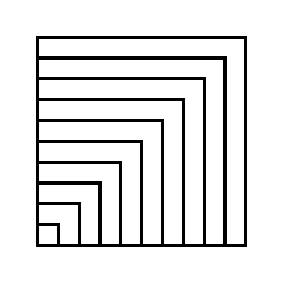
\includegraphics[width=6cm]{Argmirescr}}{Russian squares}\label{exo:russianSquaressimple}
Build the squares of different sizes as shown on figure on the right.
\end{exofigwithsizeandtitle}

\begin{exofigwithsizeandtitle}[0.35]{\includegraphics[width=4cm]{cubesandpyramid}\ \includegraphics[width=5cm]{damier}}{Spirale}\label{exo:spiralsimple}
Define two scripts that create the constructions shown on the right. Note that this task is a bit difficult and that there are different ways to solve it.
\end{exofigwithsizeandtitle}

\begin{exofigwithsizeandtitle}[0.5]{\includegraphics[width=6cm]{corridor}}{Corridor}\label{exo:corridorsimple}
Build the squares of different sizes as shown on figure on the right.
\end{exofigwithsizeandtitle}




\ifx\wholebook\relax\else
\end{document}\fi
